\documentclass[11pt]{beamer}
\gdef\pathtomaster{_LaTeX_master}
%-- Nummerierung bis Subsubsection für Report
\setcounter{secnumdepth}{3}	% zählt auch subsubsection
\setcounter{tocdepth}{3}	% Inhaltsverzeichnis bis in subsubsection

% LuaLaTeX Unterscheidung
\usepackage{ifluatex}

% Input inkl. Umlaute, Silbentrennung
\ifluatex
	\usepackage{fontspec}
\else
	\usepackage[utf8]{inputenc}
	\usepackage[T1]{fontenc}
\fi
\usepackage[english,ngerman]{babel}
\usepackage{csquotes}	% Anführungszeichen
\usepackage{marvosym}
\usepackage{eurosym}

% Style-Aufhübschung
\usepackage{soul, color}	% Kapitälchen, Unterstrichen, Durchgestrichen usw. im Text
%\usepackage{titleref}
\usepackage[breakwords, fit]{truncate}	% Abschneiden von Sätzen
\renewcommand{\TruncateMarker}{\,…}
\usepackage{setspace}

% Mathe usw.
\usepackage{amssymb}
\usepackage{amsthm}
\makeatletter%
\@ifclassloaded{beamer}%
  {}%
  {\usepackage[fleqn,intlimits]{amsmath}}%
\makeatother%
%\usepackage{mathtools} % u.a. schönere underbraces
\usepackage{xcolor}
\usepackage{esint}	% Schönere Integrale, \oiint vorhanden
\everymath=\expandafter{\the\everymath\displaystyle}	% Mathe Inhalte werden weniger verkleinert
\usepackage{wasysym}	% mehr Symbole, bspw \lightning
%\renewcommand{\int}{\int\limits}
%\usepackage{xfrac}	% mehr fracs: sfrac{}{}
\let\oldemptyset\emptyset	% schöneres emptyset
\let\emptyset\varnothing
%\RequirePackage{mathabx}	% mehr Symbole
\mathchardef\mhyphen="2D	% Hyphen in Math
\usepackage{mathtools}		% zum Beispiel {pmatrix}[r] für Formatierung der Matrix

% tikz usw.
\usepackage{tikz}
\usepackage{pgfplots}
\pgfplotsset{compat=1.11}	% Umgeht Fehlermeldung
\usetikzlibrary{graphs}
%\usetikzlibrary{through}	% ???
\usetikzlibrary{arrows}
\usetikzlibrary{arrows.meta}	% Pfeile verändern / vergrößern: \draw[-{>[scale=1.5]}] (-3,5) -> (-3,3);
\usetikzlibrary{automata,positioning} % Zeilenumbruch im Node node[align=center] {Text\\nächste Zeile} automata für Graphen
\usetikzlibrary{matrix}
\usetikzlibrary{patterns}	% Schraffierte Füllung
\usetikzlibrary{shapes.geometric}	% Polygon usw.
\tikzstyle{reverseclip}=[insert path={	% Inverser Clip \clip
	(current page.north east) --
	(current page.south east) --
	(current page.south west) --
	(current page.north west) --
	(current page.north east)}
% Nutzen: 
%\begin{tikzpicture}[remember picture]
%\begin{scope}
%\begin{pgfinterruptboundingbox}
%\draw [clip] DIE FLÄCHE, IN DER OBJEKT NICHT ERSCHEINEN SOLL [reverseclip];
%\end{pgfinterruptboundingbox}
%\draw DAS OBJEKT;
%\end{scope}
%\end{tikzpicture}
]	% Achtung: dafür muss doppelt kompliert werden!
\usepackage{graphpap}	% Grid für Graphen
\tikzset{every state/.style={inner sep=2pt, minimum size=2em}}
\usetikzlibrary{mindmap, backgrounds}
%\usepackage{tikz-uml}	% braucht Dateien: http://perso.ensta-paristech.fr/~kielbasi/tikzuml/

% Tabular
\usepackage{longtable}	% Große Tabellen über mehrere Seiten
\usepackage{multirow}	% Multirow/-column: \multirow{2[Anzahl der Zeilen]}{*[Format]}{Test[Inhalt]} oder \multicolumn{7[Anzahl der Reihen]}{|c|[Format]}{Test2[Inhalt]}
\renewcommand{\arraystretch}{1.3} % Tabellenlinien nicht zu dicht
\usepackage{colortbl}
\arrayrulecolor{gray}	% heller Tabellenlinien
\usepackage{array}	% für folgende 3 Zeilen (für Spalten fester breite mit entsprechender Ausrichtung):
\newcolumntype{L}[1]{>{\raggedright\let\newline\\\arraybackslash\hspace{0pt}}m{\dimexpr#1\columnwidth-2\tabcolsep-1.5\arrayrulewidth}}
\newcolumntype{C}[1]{>{\centering\let\newline\\\arraybackslash\hspace{0pt}}m{\dimexpr#1\columnwidth-2\tabcolsep-1.5\arrayrulewidth}}
\newcolumntype{R}[1]{>{\raggedleft\let\newline\\\arraybackslash\hspace{0pt}}m{\dimexpr#1\columnwidth-2\tabcolsep-1.5\arrayrulewidth}}
\usepackage{booktabs}	% Kompatibilität für array und \hrule
\usepackage{caption}	% Um auch unbeschriftete Captions mit \caption* zu machen

% Nützliches
\usepackage{verbatim}	% u.a. zum auskommentieren via \begin{comment} \end{comment}
\usepackage{tabto}	% Tabs: /tab zum nächsten Tab oder /tabto{.5 \CurrentLineWidth} zur Stelle in der Linie
\NumTabs{6}	% Anzahl von Tabs pro Zeile zum springen
\usepackage{listings} % Source-Code mit Tabs
\usepackage{lstautogobble} 
\makeatletter%
\@ifclassloaded{beamer}%
  {}%
  {%
\usepackage{enumitem}	% Anpassung der enumerates
%\setlist[enumerate,1]{label=(\arabic*)}	% global andere Enum-Items
\renewcommand{\labelitemiii}{$\scriptscriptstyle ^\blacklozenge$}}%
\makeatother%
\usepackage{letltxmacro} % neue Definiton von Grundbefehlen
% Nutzen:
%\LetLtxMacro{\oldemph}{\emph}
%\renewcommand{\emph}[1]{\oldemph{#1}}
\RequirePackage{xpatch}	% ua. Konkatenieren von Strings/Variablen (etoolbox)
\usepackage{xstring}	% String Operationen
\usepackage{minibox}	% Minibox anstatt \fbox{} für Boxen mit (manuellen) Zeilenumbruch
\usepackage{framed}		% \begin{framed} statt minibox/fbox mit automatischem Zeilenumbruch
\usepackage{microtype}	% Verfeinerte Hyphenation
\usepackage{import}		
\usepackage{standalone}	% Zusammen mit import: Einfügen von separaten Latex-Dateien (die schon header haben)

% Einrichtung von lst
%\renewcommand*{\ttdefault}{qcr}
\lstset{
basicstyle=\ttfamily, 
%basicstyle=\footnotesize\sffamily\color{black},
%mathescape=true, 
%escapeinside=^^, 
autogobble, 
tabsize=2,
frame=single,
rulecolor=\color{lightgray},
numbers=left,
numbersep=5pt,
numberstyle=\tiny\color{gray},
commentstyle=\color{gray},
keywordstyle=\color{htwblue},
stringstyle=\color{htworange},
morecomment=[l][\color{magenta}]{\#}
showspaces=false,
showstringspaces=false,
breaklines=true,
literate=%
    {Ö}{{\"O}}1
    {Ä}{{\"A}}1
    {Ü}{{\"U}}1
    {ß}{{\ss}}1
    {ü}{{\"u}}1
    {ä}{{\"a}}1
    {ö}{{\"o}}1
    {„}{{\glqq}}1
    {“}{{\grqq}}1
    {~}{{\textasciitilde}}1
}
\usepackage{scrhack} % Fehler umgehen
\def\ContinueLineNumber{\lstset{firstnumber=last}} % vor lstlisting. Zum wechsel zum nicht-kontinuierlichen muss wieder \StartLineAt1 eingegeben werden
\def\StartLineAt#1{\lstset{firstnumber=#1}} % vor lstlisting \StartLineAt30 eingeben, um bei Zeile 30 zu starten
\let\numberLineAt\StartLineAt

\makeatletter%
\@ifclassloaded{beamer}%
  {}%
  {
% BibTeX
\usepackage[
%backend=bibtex8,
bibencoding=ascii,
%style=authortitle, citestyle=authortitle-ibid,
%doi=false,
%isbn=false,
%url=false
]{biblatex}	% BibTeX
\usepackage{makeidx}
%\makeglossary
%\makeindex
}%
\makeatother%

% Grafiken
\usepackage{graphicx}
\usepackage{epstopdf}	% eps-Vektorgrafiken einfügen
\usepackage{transparent}	% transparent nutzen: {\transparent{0.4} ...}
%\epstopdfsetup{outdir=\customDir}
% Prüft, ob Grafik existiert (mit \ifvalidimage{}{}) [Quelle: https://tex.stackexchange.com/a/99176]:
\makeatletter
\newif\ifgraphicexist
\catcode`\*=11
\newcommand\ifvalidimage[1]{%
    \begingroup
    \global\graphicexisttrue
    \let\input@path\Ginput@path
    \filename@parse{#1}%
    \ifx\filename@ext\relax
    \@for\Gin@temp:=\Gin@extensions\do{%
        \ifx\Gin@ext\relax
        \Gin@getbase\Gin@temp
        \fi}%
    \else
    \Gin@getbase{\Gin@sepdefault\filename@ext}%
    \ifx\Gin@ext\relax
    \global\graphicexistfalse
    \def\Gin@base{\filename@area\filename@base}%
    \edef\Gin@ext{\Gin@sepdefault\filename@ext}%
    \fi
    \fi
    \ifx\Gin@ext\relax
    \global\graphicexistfalse
    \else 
    \@ifundefined{Gin@rule@\Gin@ext}%
    {\global\graphicexistfalse}%
    {}%
    \fi  
    \ifx\Gin@ext\relax 
    \gdef\imageextension{unknown}%
    \else
    \xdef\imageextension{\Gin@ext}%
    \fi 
    \endgroup 
    \ifgraphicexist
    \expandafter \@firstoftwo
    \else
    \expandafter \@secondoftwo
    \fi 
} 
\catcode`\*=12
\makeatother
\LetLtxMacro{\forceincludegraphics}{\includegraphics}	% neuer Befehl für includegraphics
\renewcommand{\includegraphics}[2][]{	% altes includegraphics neu definieren, damit es auch nicht vorhandene einfügt
\ifvalidimage{#2}{
\forceincludegraphics[#1]{#2}
}{
\message{Achtung: Grafik wurde nicht gefunden: '#2'}
\minibox[frame]{
\textbf{\StrSubstitute{#2}{_}{\_}}%  \ifthenelse{\isempty{#1}}{}{\\\textit{#1}}
}}}

% pdf-Setup
\usepackage{pdfpages}

\makeatletter
\@ifclassloaded{beamer}%
  {}%
  {\usepackage[bookmarks,
  bookmarksopen=false,
  colorlinks=true,
  linkcolor=black,
  citecolor=red,
  urlcolor=black]{hyperref}
% Nach Dokumentenbeginn ausführen:
\makeatletter
\AtBeginDocument{	
	% pdf Informationen
	\hypersetup{
		pdfauthor={\@author},
		pdftitle={\@title},
		pdfproducer={LaTeX Layout erstellt von Falk-Jonatan Strube}
	}
}
\makeatother
}%
\makeatother%



%%% ==================================================
%%% ===================== MACROS =====================
%%% ==================================================
% Horizontale Linie:
\newcommand{\HRule}[1][\medskipamount]{\par
  \vspace*{\dimexpr-\parskip-\baselineskip+#1}
  \noindent\rule[0.2ex]{\linewidth}{0.2mm}\par
  \vspace*{\dimexpr-\parskip-.5\baselineskip+#1}}
% Gestrichelte horizontale Linie:
\RequirePackage{dashrule}
\newcommand{\HDRule}[1][\medskipamount]{\par
  \vspace*{\dimexpr-\parskip-\baselineskip+#1}
  \noindent\hdashrule[0.2ex]{\linewidth}{0.2mm}{1mm} \par
  \vspace*{\dimexpr-\parskip-.5\baselineskip+#1}}
% Mathe in Anführungszeichen:
\newsavebox{\mathbox}\newsavebox{\mathquote}
\makeatletter
\newcommand{\mq}[1]{% \mathquotes{<stuff>}
  \savebox{\mathquote}{\text{"}}% Save quotes
  \savebox{\mathbox}{$\displaystyle #1$}% Save <stuff>
  \raisebox{\dimexpr\ht\mathbox-\ht\mathquote\relax}{"}#1\raisebox{\dimexpr\ht\mathbox-\ht\mathquote\relax}{''}
}
\makeatother

% Paragraph mit Zähler (Section-Weise)
\newcounter{cparagraphC}
\newcommand{\cparagraph}[1]{
\stepcounter{cparagraphC}
\paragraph{\thesection{}-\thecparagraphC{} #1}
%\addcontentsline{toc}{subsubsection}{\thesection{}-\thecparagraphC{} #1}
\label{\thesection-\thecparagraphC}
}
\makeatletter
\@addtoreset{cparagraphC}{section}
\makeatother


% (Vorlesungs-)Folien einbinden:
\makeatletter
% Folien-Pfad (inkl. Dateiname ohne Endung und ggf. ohne Nummerierung)
\newcommand{\@slidePath}{}
\newcommand{\slidePath}[1]{\renewcommand{\@slidePath}{#1}}
% Folien Eigenschaften
\newcommand{\@slideScale}{0.5}
\newcommand{\slideScale}[1]{\renewcommand{\@slideScale}{#1}}
\AtBeginDocument{
% Folien von einer Datei skaliert
\newcommand{\slide}[2][\@slideScale]{\slides[#1]{}{#2}}
\newcommand{\slideTrim}[6][\@slideScale]{\slides[#1 , clip,  trim = #5cm #4cm #6cm #3cm]{}{#2}}
% Folien von mehreren nummerierten Dateien skaliert
\newcommand{\slides}[3][\@slideScale]{\begin{center}
\includegraphics[page=#3, scale=#1]{\@slidePath #2.pdf}
\end{center}}
}
\makeatother

% \emph{} anders definieren
%\makeatletter
%\DeclareRobustCommand{\em}{%
%  \@nomath\em \if b\expandafter\@car\f@series\@nil
%  \normalfont \else \scshape \fi}
%\makeatother

% unwichtiges
\newcommand{\unimptnt}[1]{{\transparent{0.5}#1}}

% alph. enumerate
\newenvironment{anumerate}{\begin{enumerate}[label=(\alph*)]}{\end{enumerate}} % Alphabetische Aufzählung

% Hanging parameters
\newcommand{\hangpara}[1]{\par\noindent\hangindent+2em\hangafter=1 #1\par\noindent}

%% EINFACHE BEFEHLE

% Abkürzungen Mathe
\newcommand{\EE}{\mathbb{E}}
\newcommand{\QQ}{\mathbb{Q}}
\newcommand{\RR}{\mathbb{R}}
\newcommand{\CC}{\mathbb{C}}
\newcommand{\NN}{\mathbb{N}}
\newcommand{\ZZ}{\mathbb{Z}}
\newcommand{\PP}{\mathbb{P}}
\renewcommand{\SS}{\mathbb{S}}
\newcommand{\cA}{\mathcal{A}}
\newcommand{\cB}{\mathcal{B}}
\newcommand{\cC}{\mathcal{C}}
\newcommand{\cD}{\mathcal{D}}
\newcommand{\cE}{\mathcal{E}}
\newcommand{\cF}{\mathcal{F}}
\newcommand{\cG}{\mathcal{G}}
\newcommand{\cH}{\mathcal{H}}
\newcommand{\cI}{\mathcal{I}}
\newcommand{\cJ}{\mathcal{J}}
\newcommand{\cM}{\mathcal{M}}
\newcommand{\cN}{\mathcal{N}}
\newcommand{\cP}{\mathcal{P}}
\newcommand{\cR}{\mathcal{R}}
\newcommand{\cS}{\mathcal{S}}
\newcommand{\cZ}{\mathcal{Z}}
\newcommand{\cL}{\mathcal{L}}
\newcommand{\cT}{\mathcal{T}}
\newcommand{\cU}{\mathcal{U}}
\newcommand{\cX}{\mathcal{X}}
\newcommand{\cV}{\mathcal{V}}
\renewcommand{\phi}{\varphi}
\renewcommand{\epsilon}{\varepsilon}
\renewcommand{\theta}{\vartheta}

% Verschiedene als Mathe-Operatoren
\DeclareMathOperator{\arccot}{arccot}
\DeclareMathOperator{\arccosh}{arccosh}
\DeclareMathOperator{\arcsinh}{arcsinh}
\DeclareMathOperator{\arctanh}{arctanh}
\DeclareMathOperator{\arccoth}{arccoth} 
\DeclareMathOperator{\var}{Var} % Varianz 
\DeclareMathOperator{\cov}{Cov} % Co-Varianz 

% Farbdefinitionen
\definecolor{red}{RGB}{180,0,0}
\definecolor{green}{RGB}{75,160,0}
\definecolor{blue}{RGB}{0,75,200}
\definecolor{orange}{RGB}{255,128,0}
\definecolor{yellow}{RGB}{255,245,0}
\definecolor{purple}{RGB}{75,0,160}
\definecolor{cyan}{RGB}{0,160,160}
\definecolor{brown}{RGB}{120,60,10}

\definecolor{itteny}{RGB}{244,229,0}
\definecolor{ittenyo}{RGB}{253,198,11}
\definecolor{itteno}{RGB}{241,142,28}
\definecolor{ittenor}{RGB}{234,98,31}
\definecolor{ittenr}{RGB}{227,35,34}
\definecolor{ittenrp}{RGB}{196,3,125}
\definecolor{ittenp}{RGB}{109,57,139}
\definecolor{ittenpb}{RGB}{68,78,153}
\definecolor{ittenb}{RGB}{42,113,176}
\definecolor{ittenbg}{RGB}{6,150,187}
\definecolor{itteng}{RGB}{0,142,91}
\definecolor{ittengy}{RGB}{140,187,38}

% Textfarbe ändern
\newcommand{\tred}[1]{\textcolor{red}{#1}}
\newcommand{\tgreen}[1]{\textcolor{green}{#1}}
\newcommand{\tblue}[1]{\textcolor{blue}{#1}}
\newcommand{\torange}[1]{\textcolor{orange}{#1}}
\newcommand{\tyellow}[1]{\textcolor{yellow}{#1}}
\newcommand{\tpurple}[1]{\textcolor{purple}{#1}}
\newcommand{\tcyan}[1]{\textcolor{cyan}{#1}}
\newcommand{\tbrown}[1]{\textcolor{brown}{#1}}

% Umstellen der Tabellen Definition
\newcommand{\mpb}[1][.3]{\begin{minipage}[t]{#1\textwidth}\vspace*{3pt}}
\newcommand{\mpe}{\vspace*{3pt}\end{minipage}}

\newcommand{\resultul}[1]{\underline{\underline{#1}}}
\newcommand{\parskp}{$ $\\}	% new line after paragraph
\newcommand{\parnl}{\unskip\parfillskip 0pt \par} % justified new line (brace line!)

% mathematische Abkürzungen
\newcommand{\corr}{\;\widehat{=}\;}
\newcommand{\mdeg}{^{\circ}}
\newcommand{\nok}[2]{\binom{#1}{#2}}	% n über k BESSER: \binom{n}{k}
\newcommand{\mtr}[1]{\begin{pmatrix}#1\end{pmatrix}}	% Matrix
\newcommand{\dtr}[1]{\begin{vmatrix}#1\end{vmatrix}}	% Determinante (Betragsmatrix)
\LetLtxMacro{\originalVec}{\vec}
\renewcommand{\vec}[1]{\underline{#1}}	% Vektorschreibweise
\newcommand{\imptnt}[1]{\colorbox{red!30}{#1}}	% Wichtiges
\newcommand{\intd}[1]{\,\mathrm{d}#1}
\newcommand{\diffd}[1]{\mathrm{d}#1}
% für Module-Rechnung: \pmod{}
\newcommand{\unit}[1]{\,\mathrm{#1}}
%\LetLtxMacro{\ntilde}{\tilde}
%\renewcommand{\tilde}{\widetilde}

% weiter Abkürzungen
\newcommand{\gdw}{genau dann wenn}
\newcommand{\lecdate}[1]{\marginpar{\small\textcolor{gray}{Vorlesung\newline #1}}}
\definecolor{htworange}{RGB}{249,155,28}	% Corporate Design orange CMYK(0/45/100/0)
\definecolor{htwblue}{RGB}{0,116,188}			% Corporate Design blau CMYK(90/50/0/0)
\definecolor{htwgrey}{RGB}{128,128,128}		% Corporate Design gray 60% Schwarz [Annahme: CMYK(0,0,0,60)]
\RequirePackage{helvet}	% Corporate Design schreibt Arial/Helvetica vor
\renewcommand{\familydefault}{\sfdefault}	% s.o.

\usenavigationsymbolstemplate{}
\setbeamercolor{author in head/foot}{fg=black}
\setbeamercolor{title}{fg=black}
\setbeamercolor{bibliography entry author}{fg=htworange!70}
%\setbeamercolor{bibliography entry title}{fg=blue} 
\setbeamercolor{bibliography entry location}{fg=htworange!60} 
\setbeamercolor{bibliography entry note}{fg=htworange!60}  
\setbeamercolor{caption name}{fg=htworange}
\setbeamercolor{frametitle}{fg=black}
\setbeamerfont{frametitle}{size=\large}
\setbeamertemplate{frametitle}{\hspace*{-.75em}\insertframetitle}

\setbeamercolor{itemize item}{fg=black,bg=white}
\setbeamercolor{enumerate item}{fg=black,bg=white}
\setbeamercolor{itemize subitem}{fg=black,bg=white}
\setbeamercolor{enumerate subitem}{fg=black,bg=white}
\setbeamercolor{itemize subsubitem}{fg=black,bg=white}
\setbeamercolor{enumerate subsubitem}{fg=black,bg=white}
\setbeamertemplate{itemize item}{$\bullet$}
\setbeamertemplate{itemize subitem}{--}
\setbeamertemplate{itemize subsubitem}{$\bullet$}
\setbeamercolor{section in toc}{fg=black,bg=white}
\setbeamertemplate{section in toc}[sections numbered]
\setcounter{tocdepth}{1}
\makeatletter
\setbeamertemplate{footline}
{
\textcolor{htwgrey}{
\hspace*{2em}
\strut\insertshortauthor \hfill
\insertshorttitle \hfill
Folie \insertframenumber{}% / \inserttotalframenumber{}
\qquad
\@date
\hspace*{2em}\vspace*{1em}}
}
\setbeamertemplate{headline}
{%
\leavevmode%
\setlength{\arrayrulewidth}{1pt}%
\hspace*{2em}	%
\begin{tabular}{p{0.63\textwidth}}%
\rule{0pt}{3em}{\normalsize%
\textbf{%
\insertsectionhead%
%\setbox0=\hbox{\subsecname\unskip}\ifdim\wd0=0pt\else%
%~--~\insertsubsectionhead%
%\fi%
\ifx\insertsubsection\empty\else%
 \ifdefempty{\subsecname}{\relax}{%
  ~--~\insertsubsectionhead%
 }%
\fi
\strut}%
}\\%
\arrayrulecolor{htworange}%
\hline%
\end{tabular}%
\begin{tabular}{l}%
\rule{0pt}{4em}%

\includegraphics[width=3.2cm]{\pathtomaster/HTW.eps}\\%
\end{tabular}%
}%
\makeatother

% Recalculate the head of head- and footlines for each frame
% (http://tex.stackexchange.com/a/61788/3323)
\usepackage{etoolbox}
\makeatletter
\pretocmd{\beamer@@@@frame}{%
  \addtocounter{framenumber}{1}%
  \beamer@calculateheadfoot%
  \addtocounter{framenumber}{-1}}{}{}
\makeatother

\author[S. Retsch \& J. Strube]{Simon Retsch\texorpdfstring{\\}{ und }Jonatan Strube}
\title{Versionsverwaltung mit git}
\date{13.12.2017}

\usepackage{pgfpages}
%\setbeameroption{show notes on second screen=right}
\setbeamercolor{section in toc}{fg=black,bg=white}
\setbeamertemplate{section in toc}[sections numbered]
\setcounter{tocdepth}{1}

\usepackage{forest}
\BeforeBeginEnvironment{frame}{\setstretch{1.5}
\note{\setstretch{1.5}}}
\newcommand\commit[2][htwgrey]{\node[commit,fill=#1,#1] (#2) {}; \node at (#2) {\small\strut};}
\newcommand\commentm[2]{\node [clabel, outer sep=3em] at (#1) {#2}}
\newcommand\commentb[2]{\node [clabel, outer sep=2.07em] at (#1) {#2}}
\newcommand\commento[2]{\node [clabel, outer sep=1.17em] at (#1) {#2}}
\newcommand\ghost[1]{\coordinate (#1);}
\newcommand\connect[3][htwgrey]{\path (#2) [draw=#1, line width=.18em] to[out=-90,in=90] (#3);}
\begin{document}

\begin{frame}[plain]
\begin{center}

\includegraphics[width=.7\textwidth]{\pathtomaster/HTW.eps}
\end{center}
\maketitle
\end{frame}

\section*{Inhalt}
\begin{frame}
\tableofcontents
\end{frame}

\section{Prinzip Versionsverwaltung}
\begin{frame}
\note{Frage: Bitte meldet euch mal wenn ihr in einem Projekt einen Fehler gemacht habt, den alten Stand aber nicht mehr herstellen konntet und einen Teil des Projektes dann nocheinmal neu machen musstet? Für diese und andere Fälle gibt es Versionsverwaltung.}

Eigenschaften:
\begin{itemize}
	\item<2-> Sicherung
	\note{Zu jeder Zeit, vorrangegangene Zustände einsehen oder wiederherstellen}
	\item<3-> Übersicht
	\note{Genaue Protokollierung aller Änderungen aller Bearbeiter}
	\item<4-> Organisation mehrerer Bearbeiter
	\note{Mehrere Bearbeiter können gleichzeitig ein einem Projekt arbeiten und Beiträge hinzufügen. Die Beiträge werden zusammengefügt. Lediglich bei Änderungen an gleichen Passagen muss selbst eingegriffen werden}
\end{itemize}
\end{frame}

%\subsection{Details}
%\begin{frame}
%Hier noch ein paar Details.
%\end{frame}
\section{Grundlagen}
\begin{frame}
Hauptbefehle:
\begin{itemize}
	\item <1->init
	\note<1>{den Aktuellen Ordner zu einem Git Repository machen}
	\item <2->add
		\note<2>{Dateien/Änderungen zu einem aktuelle commit hinzufügen}
	\item <3->commit
		\note<3>{}
	\item <4->push
	\item <5->pull
	\item <6->merge
\end{itemize}
\end{frame}
\begin{frame}
	
\includegraphics[scale=0.3]{Bilder/git_graph1}
	\note{Beispiel eines git Projektverlaufes}
\end{frame}
\begin{frame}
	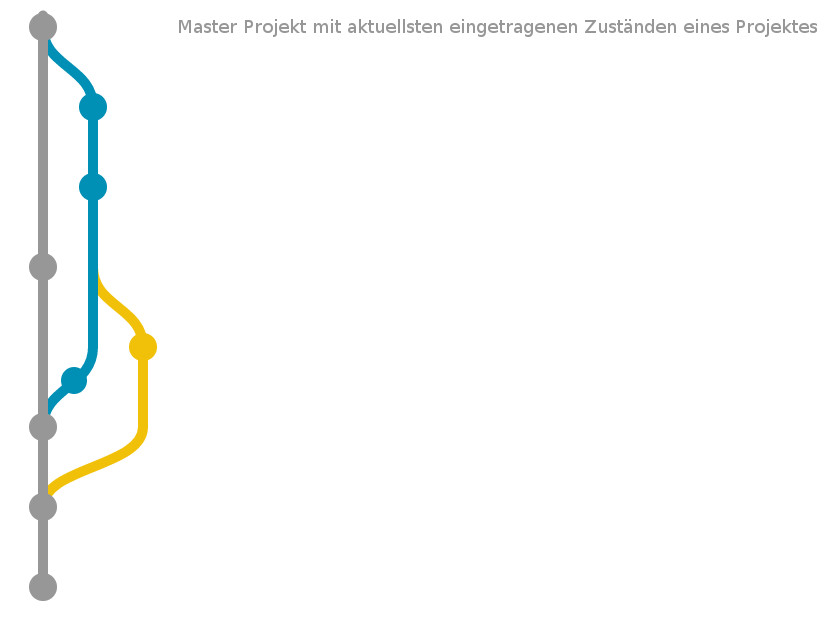
\includegraphics[scale=0.3]{Bilder/git_graph2}
	\note{Graue Linie: Master Projekt mit aktuellsten Änderungen. Alles geht zurück auf das Master Projekt. Es existiert immer nur ein Projekt mit dem interagiert wird.}
\end{frame}
\begin{frame}
	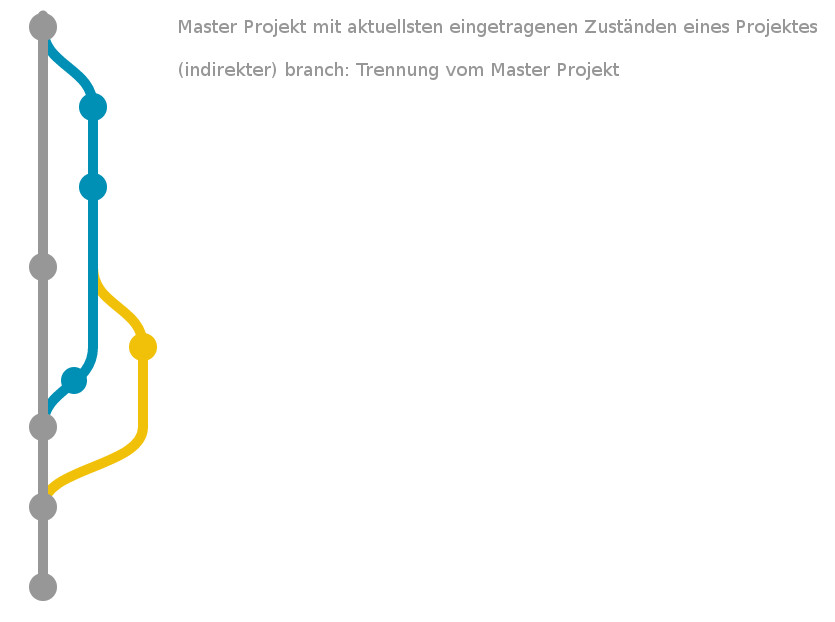
\includegraphics[scale=0.3]{Bilder/git_graph3}
	\note{Bei einer Änderung wird ein indirekter Branch einer Projektes erstellt, wie zum Beispiel bei einem...(commit)}
\end{frame}
\begin{frame}
	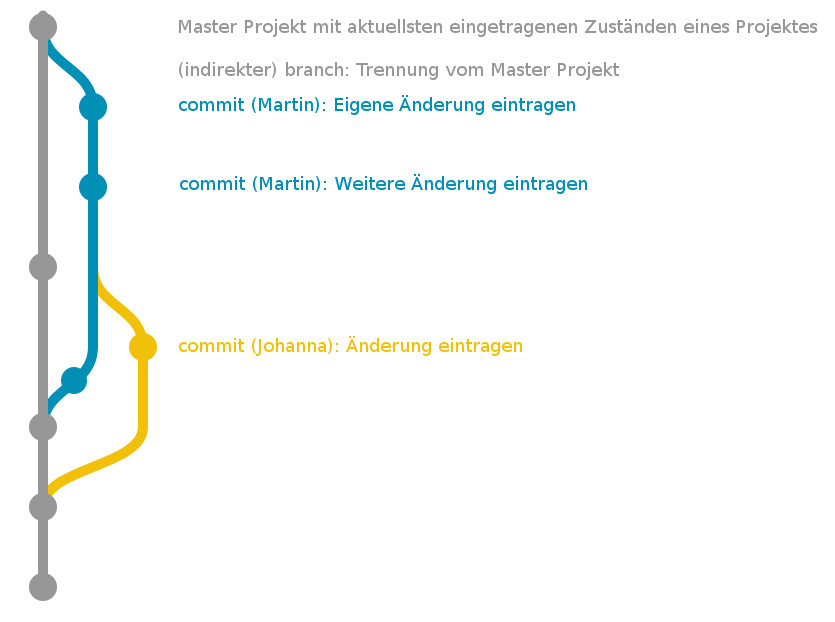
\includegraphics[scale=0.3]{Bilder/git_graph4}
	\note{Commits sind eingetragene Änderungen. Diese Einträge sollten immer einen Titel haben der die Änderungen beschreiben. Dabei sollte man eine Struktur einhalten, mehr dazu später. Vorsicht: Nach dem eine Änderung commited wurde ist sie noch nicht im Master Projekt zu finden. Dafür müssen die Änderungen...(push)}
\end{frame}
\begin{frame}
	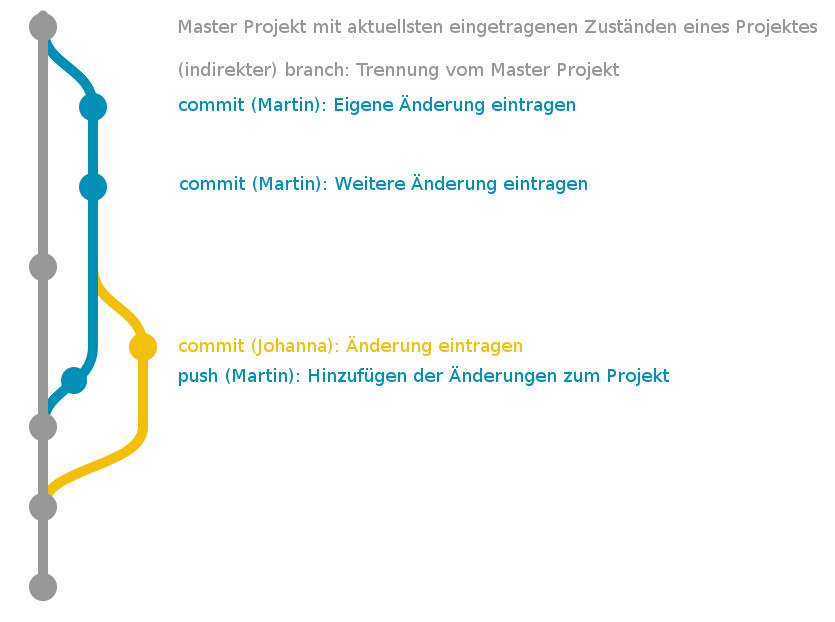
\includegraphics[scale=0.3]{Bilder/git_graph5}
	\note{Mit einem push leitet man den Vorgang ein, die noch temporären Änderungen nun einzutragen}
\end{frame}
\begin{frame}
	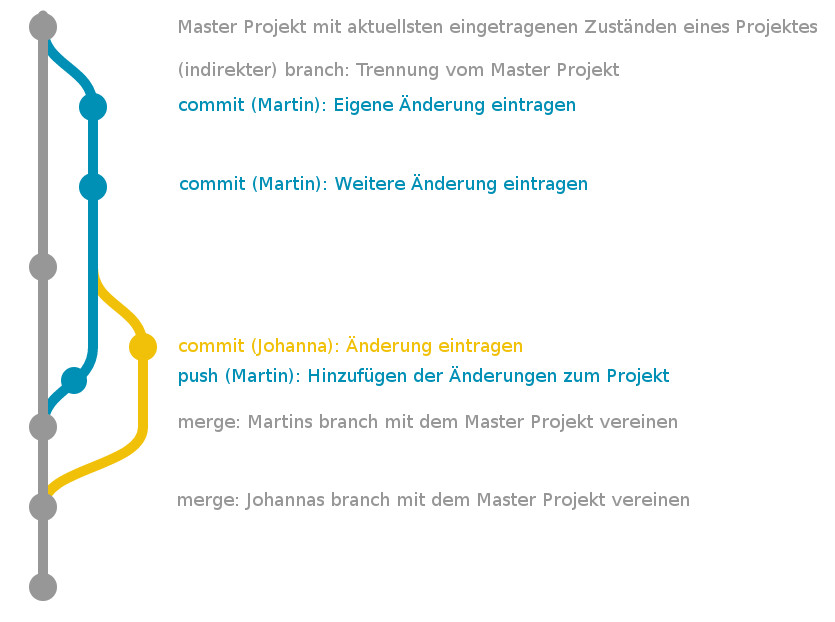
\includegraphics[scale=0.3]{Bilder/git_graph6}
	\note{Beim zusammenführen der Dateien zum Master Projekt wird ein merge gemacht, damit sind nun die Änderungen in das Master Projekt eingetragen worden}
\end{frame}
\subsection{Details}
\begin{frame}
Hier noch ein paar Details.
\end{frame}
\subsection{gitignore}
\begin{frame}
\uncover<2->{Versionierung sinnvoll bei:}
\begin{itemize}
\item<3-> Textdateien
\end{itemize}
\uncover<4->{Nicht sinnvoll bei:}
\begin{itemize}
\item<5-> Binärdateien
\end{itemize}
\end{frame}

\begin{frame}
\begin{itemize}
\item<1-> Schwarze Liste von Dateien/Ordnern
\begin{itemize}
\item<2-> Binäres \hfill \lstinline`*.exe`
\item<3-> Von Programmen \hfill \lstinline`.vscode/`
\item<4-> Geheimes \hfill \lstinline`my_password.txt`
\end{itemize}
\item<5-> Weiße Liste
\begin{itemize}
\item<6-> Ausnahmen zur schwarzen Liste mit \lstinline`!` \hfill \lstinline`!final/*`
\end{itemize}
\end{itemize}
\note<2>[item]{regex Charakter}
\note<6>[item]{Ausnahme zur schwarzen Liste hinter schwarzer Liste!}
\end{frame}

\begin{frame}[fragile]
\setstretch{1}
Datei \lstinline`.gitignore`:
\begin{lstlisting}[numbers=none, language=python]
# alle Binärdateien:
*.exe
*.out
# Ordner von VSC:
.vscode/
# Geheimes:
mein_passwort.txt
bildchen/*
# Behalte Einzeldatei:
!bildchen/goodprof.png
\end{lstlisting}
\end{frame}

\begin{frame}[fragile]
\setstretch{1}
\note[item]{.git beinhaltet alle Informationen zum Repository und wird selbst verständlich ignoriert}
\begin{center}
\begin{minipage}{.3\textwidth}
\tiny
\begin{lstlisting}[numbers=none, language=python]
# alle Binärdateien:
*.exe
*.out
# Ordner von VSC:
.vscode/
# Geheimes:
mein_passwort.txt
bildchen/*
# Behalte Einzeldatei:
!bildchen/goodprof.png
\end{lstlisting}
\end{minipage}
\qquad
\begin{minipage}{.3\textwidth}
%\scalebox{.65}{
\tiny
\begin{forest}
  for tree={
    font=\ttfamily,
    grow'=0,
    child anchor=west,
    parent anchor=south,
    anchor=west,
    calign=first,
    edge path={
      \noexpand\path [draw, \forestoption{edge}]
      (!u.south west) +(7.5pt,0) |- node[fill,inner sep=1.25pt] {} (.child anchor)\forestoption{edge label};
    },
    before typesetting nodes={
      if n=1
        {insert before={[,phantom]}}
        {}
    },
    fit=band,
    before computing xy={l=15pt},
  }
[repository/
	[{\color{htwgrey}.git/}]
  [{\only<5>{\color{htworange}}%
  \only<6>{\color{htwblue}}bildchen/}
    [{\only<5->{\color{htwgrey}}badprof.png}]
    [{\only<5-6>{\color{htwgrey}}\only<6>{\color{htwblue}}goodprof.png}]
  ]
  [programm/
  	[{\only<4->{\color{htwgrey}}\only<3>{\color{htworange}}.vscode/}
			[{\only<3->{\color{htwgrey}}…}]  	
  	]
    [readme.md]
    [virus.c]
    [{\only<2->{\color{htwgrey}}virus\_unix%
    {\only<2>{\color{htworange}}.out}}]
    [{\only<2->{\color{htwgrey}}virus\_win%
    {\only<2>{\color{htworange}}.exe}}]
  ]
  [.gitignore]
  [deren\_passwoerter.txt]
  [{\only<5->{\color{htwgrey}}\only<4>{\color{htworange}}mein\_passwort.txt}]
  [{\only<2->{\color{htwgrey}}no\_virus%
  {\only<2>{\color{htworange}}.exe}}]
  [virus.png]
]
\only<7>{}
\end{forest}
%}
\end{minipage}
\end{center}
\end{frame}

\subsection{Commit Nachricht Richtlinien}
\begin{frame}
\uncover<2->{Commit Nachricht besteht aus:}
\begin{itemize}
\item<3-> Thema / Titel (\emph{subject})\\
\uncover<5->{Kurze Beschreibung.}
\item<4-> Rumpf / Beschreibung (\emph{body})\\
\uncover<6->{\emph{Was} wurde \emph{warum} geändert (nicht \emph{wie})}
\end{itemize}
\end{frame}

\begin{frame}{Richtlinien Titel}
\begin{itemize}
\item<2-> Kurz (50, max. 72 Zeichen)
\note<2>[item]{viele GUIs schneiden längere Titel ab}
\item<3-> Mit Großbuchstabe beginnen
\item<4-> Kein Punkt am Ende
\item<5-> Imperativ
\note<5>{Im Englischen: If applied, this commit will ...\\
Positiv: If applied, this commit will remove deprecated methods
Negativ: If applied, this commit will more fixes for broken stuff
}
\end{itemize}
\end{frame}

\begin{frame}{Negativbeispiel}
\footnotesize

\texttt{\noindent
Erweiterung Keylogger, der alles Aufgezeichnete in eine Datei im selben Ordner speichert.\bigskip\\
Es wurde ein Keylogger durch memory injection implementiert. In Zeilen 50-100 der Codedatei kann man gut sehen, wie die durch einen buffer overflow jedes Betriebssystem komprimiert werden kann.\\
Mehr Passwörter! Yay.
}
\end{frame}

\begin{frame}{Beispielnachricht}
\footnotesize

\texttt{\noindent
Erweitere Virus um Keylogger\bigskip\\
Es wurde ein Keylogger implementiert, der alle 
Nutzereingaben aufzeichnet und speichert.\\
Dadurch können mehr Passwörter ausgelesen werden.
}
\end{frame}



\section{Anbieter}
\begin{frame}
Hier steht was zu Anbietern.
\end{frame}

\subsection{Details}
\begin{frame}
Hier noch ein paar Details.
\end{frame}
\section{Apps}
\begin{frame}
\begin{itemize}
	\item SourceTree
	\item GitHub Desktop
	\item Integriert in Visual Studio Code
\end{itemize}
\end{frame}

\subsection{SourceTree}
\begin{frame}{„einfach und mächtig“}
\begin{itemize}
\item Selbsterklärendes GUI
\item Auch erweiterte Funktionalitäten über GUI:\\
cherry picking, checkout älterer commits, …
\end{itemize}
\end{frame}

\subsection{GitHub Desktop}
\begin{frame}
\begin{itemize}
\item Sehr eingeschränkte Funktionalität
\item Für Alltag ausreichend
\end{itemize}
\end{frame}

\subsection{Visual Studio Code}
\begin{frame}
Features:
\begin{itemize}
	\item <2->Einbindung in Entwicklungsumgebung
	\begin{itemize}
		\item <3->Direkter Import (clone) von Git Repositories
		\item <4->push, pull, add, commit direkt in IDE
		\item <5->Automatische checkouts
		\note{beim Rückgängig machen}
	\end{itemize}
	\item <6->Anzeige aktuell geänderter Passagen im Editor
\end{itemize}
\end{frame}
\section{Vorführung}
\begin{frame}
\setstretch{1}
Vorführung zeigt git-Nutzung in Visual Studio Code:
\begin{itemize}
\item Veranschaulichung:
\begin{itemize}
\item \emph{Pull}
\item \emph{Commit}
\item \emph{Push}
\end{itemize}
\item Konflikte Lösen bei parallelem Bearbeiten\\
(ohne \emph{pull} vor \emph{commit})
\item In anderem \emph{branch} wechseln/arbeiten und\\
zurück wechseln (\emph{Checkout})
\item \emph{Branch} zum \emph{master} mergen
\end{itemize}
\end{frame}

\section*{Quellen}
\begin{frame}
\setstretch{1}
\tiny
Prinzip
\begin{itemize}
\item N/A
\end{itemize}
Grundlagen
\begin{itemize}
\item \url{https://gist.github.com/robertpainsi/b632364184e70900af4ab688decf6f53}
\item \url{https://wiki.openstack.org/wiki/GitCommitMessages}
\item \url{https://chris.beams.io/posts/git-commit/}
\end{itemize}
Anbieter
\begin{itemize}
\item \url{https://medium.com/flow-ci/github-vs-bitbucket-vs-gitlab-vs-coding-7cf2b43888a1}
\end{itemize}
Apps
\begin{itemize}
\item
\end{itemize}
Vorführung
\begin{itemize}
\item N/A
\end{itemize}
\end{frame}

%{
%\setbeamercolor{background canvas}{bg=}
%\makeatletter
%\@latex@warning{ACHTUNG: Vor dem Kompilieren dieser Praesentation muessen alle anderen pdfs kompiliert werden!!!}
%\@latex@warning{Diese .tex Datei fuegt die pdfs nur aneinander!}
%\makeatother
%\includepdf[pages={-}]{Abschlusspraesentation_Projektmanager.pdf}
%\includepdf[pages={-}]{Abschlusspraesentation_Analysierender.pdf}
%\includepdf[pages={-}]{Abschlusspraesentation_Entwerfender.pdf}
%\includepdf[pages={-}]{Abschlusspraesentation_Datenbankender.pdf}
%\includepdf[pages={-}]{Abschlusspraesentation_Implementierender.pdf}
%\includepdf[pages={-}]{Abschlusspraesentation_Testender.pdf}
%\includepdf[pages={-}]{Abschlusspraesentation_Dokumentierender.pdf}
%\includepdf[pages={-}]{Abschlusspraesentation_Qualitätsmanager.pdf}
%}

\end{document}